\documentclass[12pt,oneside,a4paper,chapter=TITLE,english,brazil,sumario=abnt-6027-2012]{abntex2}

\usepackage{../sub/tcc_style}

\titulo{\bfseries MATRIZ DE CORRELAÇÃO ENTRE AS QUATRO PRINCIPAIS LIGAS DE ESPORTES DOS ESTADOS UNIDOS}

\autor{GUILHERME DE MORAES MASUKO}



\local{RIO DE JANEIRO/ RIO DE JANEIRO}
\data{\the\year}
\tipotrabalho{artigo}
\instituicao{Pontifícia Universidade Católica - Rio de Janeiro (PUC-Rio)}




\begin{document}
	
\clearpage\maketitle
\thispagestyle{empty}
\setlength{\absparsep}{18pt} 
\begin{resumo}
	
	
	\noindent
	
	\textbf{Palavras-chave}:  Correlação. Esporte.   
\end{resumo}


	
	\pdfbookmark[0]{\contentsname}{toc}
	\tableofcontents*
	\cleardoublepage
	
	
	
	\textual 
	\pagestyle{simple}
	\aliaspagestyle{chapter}{simple}
	
\chapter{Introdução}

	Os Estados Unidos é um país conhecido pelo seu ótimo desempenho no esporte. Entre os esportes mais populares, estão o futebol americano, basquete, hóquei e beisebol. O Super Bowl é 
	


\chapter{Metodologia}

	Para mensurar a relação entre a performance média das regiões metropolitanas nas ligas norte-americana NBA, MLB e NFL, será proposto como medidor de performance, visualizado na equação \ref{perf}, a razão entre vitórias e jogos de cada time, ou seja
	
	\begin{equation}
		P_i = \frac{W_i}{G_i}
		\label{perf}
	\end{equation}
	onde $P_i$ é a performance do time $i$, $W_i$ é a quantidade de vitórias na temporada regular do time $i$ e $G_i$ é a quantidade de jogos da temporada regular do time $i$.
	
	Para a liga NHL, como há um esquema de pontuação diferente, onde o time ganha dois pontos caso vença, um ponto caso seja derrotado em um overtime, e zero caso seja derrotado no tempo normal, o medidor de performance é proposto a partir da razão entre pontuação do time e pontuação possível, este último travado em 164 (pontuação caso um time ganhar as 82 partidas que contém uma temporada regular). A equação \ref{perf_nhl} ilustra isso.
	
	\begin{equation}
		P_i = \frac{Pt_i}{\mbox{max}(Pt)} = \frac{Pt_i}{164}
		\label{perf_nhl}
	\end{equation}
	onde $P_i$ é a performance do time $i$, $Pt_i$ é a pontuação na temporada regular do time $i$ e $\mbox{max}(Pt)$ é a pontuação máxima, de 164 pontos, da temporada regular que um time pode atingir.
	
	Possivelmente vários times podem estar situados em mesma região metropolitana e para chegar na performance da região será utilizado a média simples da performance de cada time.
	
	E, finalmente, para mensurar a relação entre a performance média das regiões metropolitanas usaremos a matriz de correlação para as quatro principais ligas norte-americanas. Como pode ser visto em \citeonline{corr}, correlação é uma medida estatística de relação (causal ou não-causal) entre duas variáveis abordando o comportamento da relação entre elas. O coeficiente de correlação utilizado pela presenta análise será o de Pearson, o coeficiente de correlação mais comumente usado. 
	
	O coeficiente de correlação de Pearson, segundo \citeonline{corr_pearson}, define o quanto e em qual direção duas variáveis estão relacionadas, sendo obtida a partir da seguinte fórmula demonstrada na equação \ref{corr} abaixo.. Usado normalmente como $\rho$, o coeficiente pode ter valores em um range de $-1$ à $1$, isto é, $-1 \leq \rho \leq 1$, onde $\rho =-1$ significa uma relação perfeitamente negativa entre as variáveis, $\rho=1$ uma relação perfeitamente positiva, e $\rho=0$ uma relação de não dependência linear (isso não diz nada sobre não haver dependência de modo geral entre as variáveis).
	
	\begin{equation}
		\rho_{X,Y} = \frac{\mbox{COV}(X,Y)}{\sqrt{\mbox{VAR}(X)}\sqrt{\mbox{VAR}(X)}}
		\label{corr}
	\end{equation}
	onde $\rho_{X,Y}$ é a correlação entre $X$ e $Y$.
	
	A matriz de correlação é uma ferramente estatística capaz de medir a correlação de uma coleção de variáveis em seus pares, uma ótima maneira de obter de forma reduzida, o comportamento de várias séries em uma só tabela. Uma matriz de correlação de $n$ variáveis $X_1$,...,$X_n$, é uma matriz $nxn$, no qual o $i$,$j$-ésimo elemento da matriz é a correlação entre $X_i$ e $X_j$, isto é, $\rho_{X_i,X_j}$.
	
	
\chapter{Dados}

Os dados das regiões metropolitanas dos Estados Unidos utilizados nesse estudo foram obtidos através de \citeonline{reg_metro}, onde uma tabela pode ser encontrada relacionando cada região metropolitana com os times da big four. Nesta tabela também há informações sobre a quantidade populacional de cada região, com dados atualizados para o ano de 2016.

A primeira liga abordada foi a Liga Nacional de Hóquei. Para esta e todas as demais ligas presentes neste trabalho, foi escolhido os resultados da temporada regular de 2018. No gráfico \ref{nhl}, podemos verificar a performance de cada time na temporada regular utilizando o medidor proposto como a razão de vitórias e jogos.

\begin{figure}[H]
	\centering
	\caption{Performance Temporada Regular National Hockey League (NHL) 2018}
	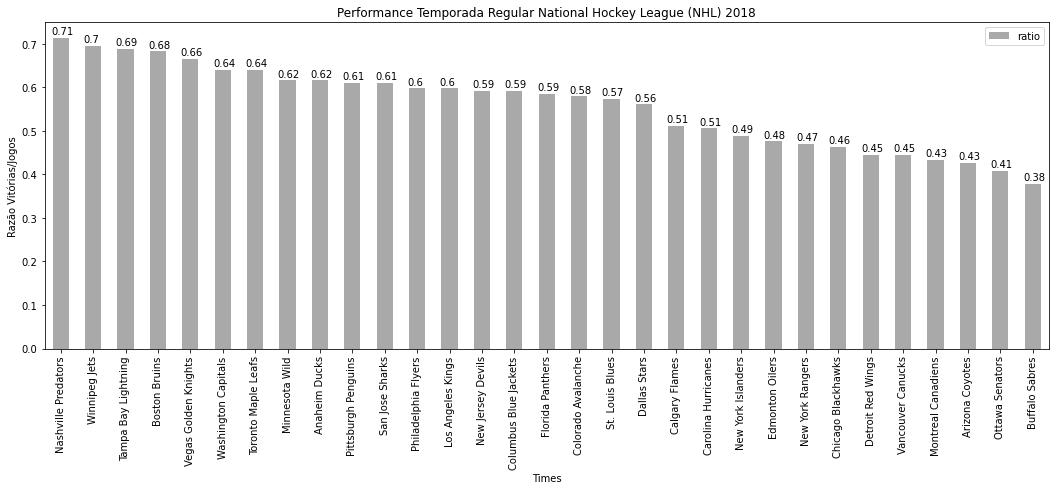
\includegraphics[scale=0.4]{../../output/figures/nhl.png}
	\label{nhl}
	\\ \vspace{0.25cm}
	\raggedright
	\footnotesize{Fonte: Elaboração própria a partir de \citeonline{nhl}}
\end{figure}

O destaque para a liga de hóquei ficou para o Nashville Predators. O time de Nashville se mostrou muito forte com uma razão de 75\% de performance. O segunda esporte analisado é o basquete, 

\begin{figure}[H]
	\centering
	\caption{Performance Temporada Regular National Basketball Association (NBA) 2018}
	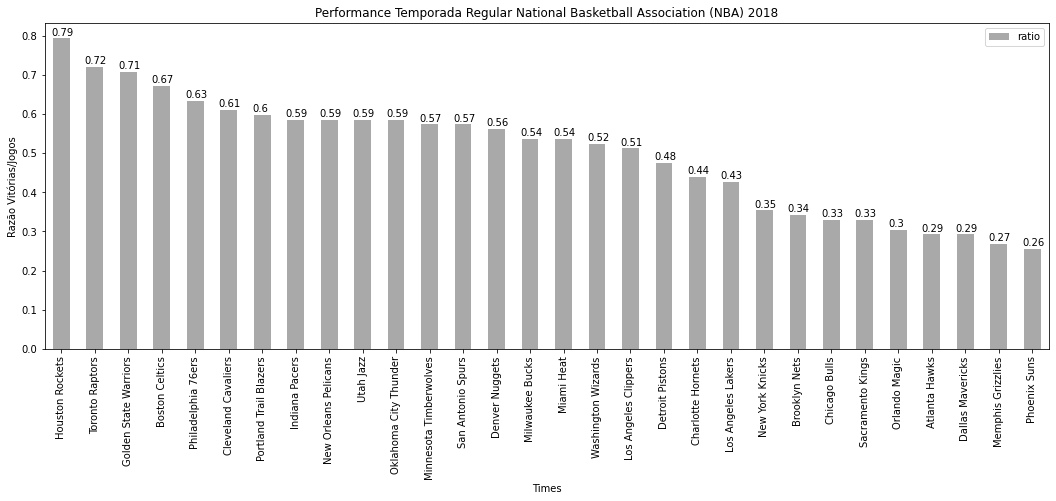
\includegraphics[scale=0.4]{../../output/figures/nba.png}
	\label{dist}
	\\ \vspace{0.25cm}
	\raggedright
	\footnotesize{Fonte: Elaboração própria a partir de \citeonline{nba}}
\end{figure}


\begin{figure}[H]
	\centering
	\caption{Performance Temporada Regular Major League Baseball (MLB) 2018}
	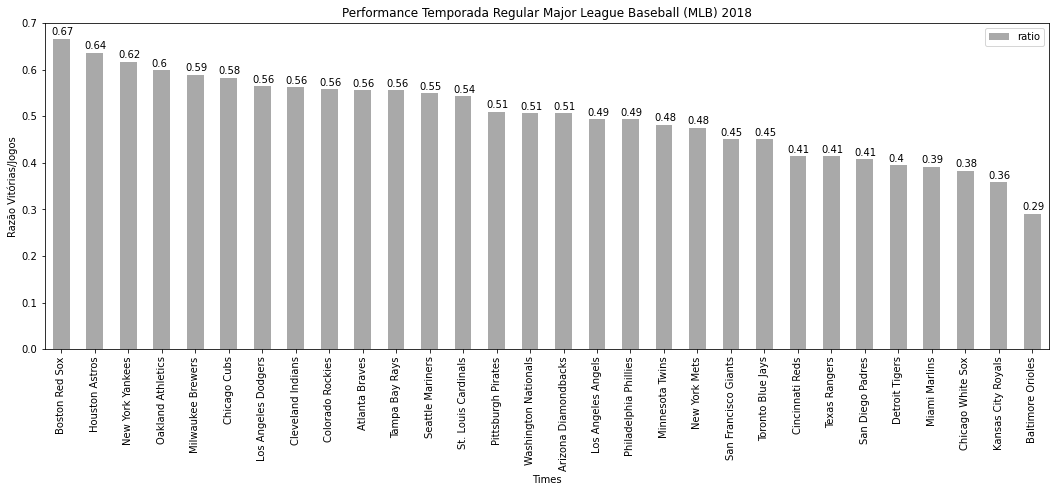
\includegraphics[scale=0.4]{../../output/figures/mlb.png}
	\label{dist}
	\\ \vspace{0.25cm}
	\raggedright
	\footnotesize{Fonte: Elaboração própria a partir de \citeonline{mlb}}
\end{figure}


\begin{figure}[H]
	\centering
	\caption{DPerformance Temporada Regular National Football League (NFL) 2018}
	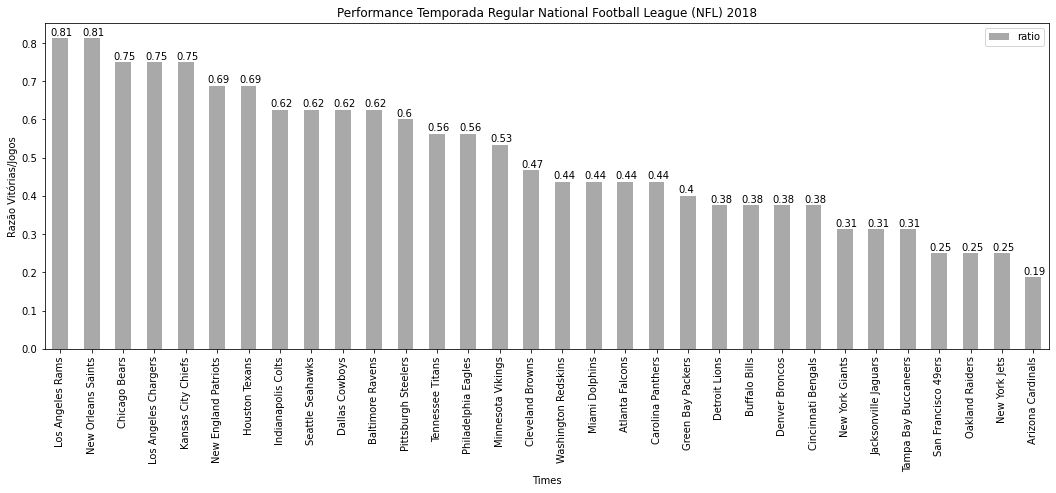
\includegraphics[scale=0.4]{../../output/figures/nfl.png}
	\label{dist}
	\\ \vspace{0.25cm}
	\raggedright
	\footnotesize{Fonte: Elaboração própria a partir de \citeonline{nfl}}
\end{figure}

	
\chapter{Conclusão}

	\begin{table}[H]
	\centering
	\begin{tabular}{lrrrr}
	& NFL & NBA & NHL & MLB \\\hline
	NFL &  & 0.237000 & 0.304000 & -0.050000 \\\hline
	NBA & 0.237000 &  & 0.760000 & 0.325000 \\\hline
	NHL & 0.304000 & 0.760000 &  & 0.432000 \\\hline
	MLB & -0.050000 & 0.325000 & 0.432000 &  \\\hline
	\end{tabular}
	\end{table}	

	
	\bibliographystyle{abntex2-alf}
	\bibliography{ref}

\end{document}
	
	